\documentclass[../main/main.tex]{subfiles}


\begin{document}

\section{September 4th, 2019}
\subsection{NP-Completeness of Finding Large Itemsets}
The problem of finding all ``large" itemsets is equivelent to finding all ``large" $J$-itemsets for each positive integer $J$. (for our case this is finding $J$-itemsets with support $\ge 3$).\\

However, this problem is NP-Complete, as it is equivelent to solving the \vocab{Balanced Complete bipartite Subgraph}, a known NP-Complete problem.

\begin{definition}
	The \vocab{Balanced Complete Bipartitie Subgraph} is as follows: 
	\begin{itemize}
		\item Instance: Given a bipartite graph $G=(V,E)$ and positive integer $K\le \left| V \right| $
	\item Question: Are there two disjoint subsets $V_1,V_2\subseteq V$ such that $\left| V_1 \right| =\left| V_2 \right| =K$ and such that, for each $u\in V_1$ and each $v\in V_2$, $(u,v)\in  E$.
	\end{itemize}
\end{definition}
	\begin{figure}[htpb]
		\centering
		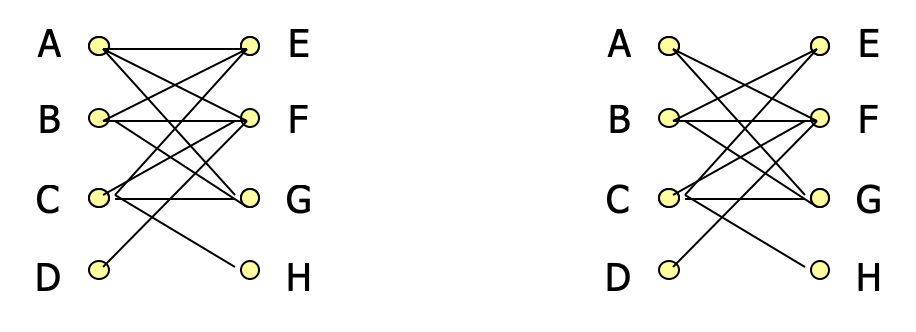
\includegraphics[width=0.8\textwidth]{9-2-bcbs.png}
		\caption{$V_1=\{A,B,C\}, V_2=\{E,F,G\} $ for the left, no such $V_1,V_2$ exists for the right}
		\label{fig:}
	\end{figure}
	The reduction from the graph problem to the itemset problem is as follows:
	\begin{itemize}
		\item For each vertex in $V_1$, create a transaction
		\item For each vertex in $V_2$, create a item
		\item For each edge $(u,v)$, create a purchase of item $v$ in transaction $u$
		\item We have $f=K$ and $J=K$
	\end{itemize}
	\begin{remark}
		In other words, solving the graph problem is equivelent tothe itemset problem, i.e. is there a $K$-frequent itemset of size $K$. Since this is a restriction of the itemset problem, if we can solve the itemset problem, we can solve the Balanced Complete Bipartite Subgraph problem. As such, the itemset problem is also NP-Complete, since BCBS is NP-Complete.
	\end{remark}
	\begin{remark}
		NP-Complete means that there is no polynomial time algorithm to solve it (unless P=NP).
	\end{remark}
	\subsection{Algorithm Aprior}
	This algorithm starts with ``large" 1-itemsets, and iteratively builds ``large" itemsets with bigger sizes (1-itemsets$\to$ 2-itemset$\to\ldots$). It can be described as follows:
	\begin{itemize}
		\item Start with $L_1=\{\{A\} ,\{B\} ,\{C\} ,\{D\} ,\{E\} \} $, i.e. the large $1$-itemsets.
		\item From $L_1$, generate candidates for large $2$-itemsets, $C_2$.
		\item From $C_2$, check and keep the large $2$-itemsets, $L_2$.
		\item Repeat
	\end{itemize}
	To generate candidates for ``large" $n$-itemsets from $L_{n-1}$, we can take note of the following properties:
	\begin{theorem}\label{largesubsets}
		If an itemset $S$ is large, then any proper subset of $S$ must be large.
	\end{theorem}
	\begin{proof}
		Note that the proper subsets of $S$ are a relaxed version of $S$. Since we are relaxing the constraint, this property must be true.
	\end{proof}
\begin{theorem}
	If an itemset $S$ is NOT large, then any proper superset of $S$ must NOT be large.
\end{theorem}
\begin{proof}
	Similarly, since the proper supersets are restricted versions of $S$, if $S$ is not large, then any proper supersets of $S$ must not be large, since it's even more restricted.
\end{proof}
\begin{example}
	$\{B,C,E\} $ is large, thus $\{B,C\} ,\{C,E\} \{C\} $ are all large (not exahstive).
\end{example}
	Using these properties, we can split the generation step into two steps: 
	Suppose we know that the itemset $B,C$ and the itemset $B,E$ are large (i.e. in $L_2$)
\end{document}

